\documentclass[12pt,a4paper]{article}

% ============================================================
% PACKAGES
% ============================================================
\usepackage[a4paper,margin=1in]{geometry}
\usepackage{times}
\usepackage{setspace}
\usepackage{graphicx}
\usepackage{float}
\usepackage{booktabs}
\usepackage{array}
\usepackage{multirow}
\usepackage{longtable}
\usepackage{tabularx}
\usepackage{amsmath,amssymb}
\usepackage{algorithm}
\usepackage{algpseudocode}
\usepackage{xcolor}
\usepackage{listings}
\usepackage{tikz}
\usepackage{pgfplots}
\usepackage{caption}
\usepackage{subcaption}
\usepackage{hyperref}
\usepackage{enumitem}
\usepackage{fancyhdr}
\usepackage{titlesec}

\usetikzlibrary{
    shapes.geometric,
    arrows.meta,
    positioning,
    fit,
    calc
}

\pgfplotsset{compat=1.18}

% ============================================================
% HYPERLINKS
% ============================================================
\hypersetup{
    colorlinks=true,
    linkcolor=blue,
    citecolor=blue,
    urlcolor=blue,
    pdftitle={Machine Learning-Based Loop Optimization for High-Performance Compiler Design}
}

% ============================================================
% LINE SPACING
% ============================================================
\onehalfspacing

% ============================================================
% HEADER / FOOTER
% ============================================================
\pagestyle{fancy}
\fancyhf{}
\fancyhead[L]{Compiler Design Lab -- CSE3024}
\fancyhead[R]{VIT-AP University}
\fancyfoot[C]{\thepage}

% ============================================================
% CODE STYLE
% ============================================================
\definecolor{codegreen}{rgb}{0,0.5,0}
\definecolor{codegray}{rgb}{0.5,0.5,0.5}
\definecolor{codepurple}{rgb}{0.58,0,0.82}

\lstset{
    language=C,
    basicstyle=\ttfamily\small,
    keywordstyle=\color{blue},
    commentstyle=\color{codegreen},
    stringstyle=\color{codepurple},
    numbers=left,
    numberstyle=\tiny\color{codegray},
    stepnumber=1,
    numbersep=8pt,
    frame=single,
    breaklines=true,
    showstringspaces=false
}

% ============================================================
% TITLE FORMAT
% ============================================================
\titleformat{\section}
{\large\bfseries}
{\thesection.}{0.5em}{}

\titleformat{\subsection}
{\normalsize\bfseries}
{\thesubsection}{0.5em}{}

% ============================================================
% DOCUMENT
% ============================================================
\newcommand{\numKernels}{182}
\newcommand{\numFamilies}{9}
\newcommand{\numConfigs}{7}
\newcommand{\numFeatures}{23}
\newcommand{\numCompiles}{1274}
\newcommand{\numRuns}{6370}
\newcommand{\cpuModel}{Intel(R) Core(TM) i5-6200U CPU @ 2.30GHz}
\newcommand{\gccVersion}{gcc (Ubuntu 13.3.0-6ubuntu2~24.04.1) 13.3.0}
\newcommand{\numCpus}{4}
\newcommand{\memGB}{3.8}
\newcommand{\noiseSpreadMedian}{28.8}
\newcommand{\noiseSpreadMean}{38.8}
\newcommand{\noiseSplitMedian}{8.6}
\newcommand{\noiseSplitNinety}{22.4}
\newcommand{\selModel}{k-NN}
\newcommand{\selAccCV}{66.5}
\newcommand{\selAccLOFO}{48.4}
\newcommand{\selFscoreCV}{0.41}
\newcommand{\selFscoreLOFO}{0.27}
\newcommand{\selGMCV}{2.221}
\newcommand{\selGMLOFO}{1.794}
\newcommand{\oracleGM}{2.316}
\newcommand{\selFracCV}{95.0}
\newcommand{\selFracLOFO}{69.6}
\newcommand{\selSlowCV}{6.0}
\newcommand{\selSlowLOFO}{12}
\newcommand{\selRegretCV}{5.0}
\newcommand{\selRegretLOFO}{64.7}
\newcommand{\gmOThree}{1.054}
\newcommand{\gmONative}{1.512}
\newcommand{\gmOFast}{2.197}
\newcommand{\fastSlow}{6}
\newcommand{\fastRegret}{6.0}
\newcommand{\fastFrac}{93.7}
\newcommand{\pOracle}{1.175}
\newcommand{\pOThree}{1.054}
\newcommand{\pOThreeSlow}{32}
\newcommand{\pCV}{1.108}
\newcommand{\pLOFO}{1.039}
\newcommand{\pFracCV}{63.5}
\newcommand{\pFracLOFO}{23.5}
\newcommand{\pSlowCV}{6.4}
\newcommand{\pSlowLOFO}{3}
\newcommand{\featMs}{0.7}
\newcommand{\predMs}{1.3}
\newcommand{\gccCompileMs}{71}


\begin{document}

% ============================================================
% PAGE 1 -- TITLE PAGE
% ============================================================
\begin{titlepage}
\begin{center}

\vspace*{0.5cm}


\includegraphics[width=3.2cm]{vit-ap-university-logo.png}

\vspace{0.3cm}

{\Large\bfseries
VIT-AP UNIVERSITY
}

\vspace{0.3cm}

{\large
Amaravati, Andhra Pradesh, India
}

\vspace{0.8cm}

{\Large\bfseries
COMPILER DESIGN LAB REPORT
}

\vspace{0.4cm}

{\large
\textbf{Subject Name: Compiler Design Lab}
}

\vspace{0.15cm}

{\large
\textbf{Course Code: CSE3024}
}

\vspace{1cm}

{\LARGE\bfseries
Machine Learning-Based Loop Optimization\\
for High-Performance Compiler Design
}

\vspace{1.2cm}

\textbf{Submitted by}

\vspace{0.4cm}

\begin{tabular}{ll}
\textbf{Poojith} & \textbf{Regd. No.:} 24BCB7244 \\[0.4cm]
\textbf{Student 2 Name} & \textbf{Regd. No.:} 24BCB7161 \\
\end{tabular}

\vspace{1.2cm}

\textbf{Under the Guidance of}

\vspace{0.3cm}

\textbf{Dr. Prakash Kumar Sarangi}

\vspace{1cm}

{\large
School of Computer Science and Engineering (SCOPE)\\
VIT-AP University\\
Amaravati, Andhra Pradesh, India
}

\vspace{0.4cm}

{\large
Academic Year 2026--2027
}

\end{center}
\end{titlepage}

% ============================================================
% PAGE 2 -- ABSTRACT
% ============================================================
\section*{Abstract}

High-performance computing programs spend most of their time in loop nests, and
the speed of the generated code depends on optimisation choices such as
vectorisation, unrolling and the use of the target instruction set. Production
compilers make these choices with fixed, hand-written heuristics that cannot
adapt to the individual loop. This report designs and evaluates an
ML-based loop-optimisation decision model that sits in front of an unmodified
GCC compiler.

A compiler front end is implemented from scratch: a lexical analyser, a
recursive-descent parser, a semantic and loop analyser, and a three-address-code
generator. From the analysed loop nest the front end computes \numFeatures\
static features, such as trip counts, exact memory strides, loop-carried
dependence distance, reductions, arithmetic intensity and working-set size. A
supervised model maps the features to one of \numConfigs\ GCC optimisation
configurations. The model is trained on \numKernels\ C loop kernels from
\numFamilies\ HPC-style families (vector updates, reductions, recurrences,
1-D/2-D stencils, matrix multiplication, 2-D traversals, branchy and strided
loops). Every kernel was compiled with every configuration (\numCompiles\
compilations) and executed on the target machine, and the label is the best
configuration that preserves the numerical result.

The evaluation uses the speed-up of the generated code. With random 5-fold
cross-validation the best model (\selModel) reaches a geometric-mean speed-up of
\selGMCV$\times$ over \texttt{-O2}, which is \selFracCV\% of the gain of the oracle
(\oracleGM$\times$). This must be compared honestly with static choices: always using
\texttt{-O3} gives \gmOThree$\times$, always using \texttt{-O3 -march=native} gives
\gmONative$\times$, and always using \texttt{-O3 -march=native -ffast-math} gives
\gmOFast$\times$. On this machine the learned model is therefore only marginally better
than the most aggressive static configuration in cross-validation, and on loop families
never seen in training (leave-one-family-out) it is worse (\selGMLOFO$\times$), which shows the
limits of a small corpus. The model is more useful when the binary must be portable and
IEEE-safe: among the four non-native, non-fast-math configurations it reaches \pCV$\times$
(oracle \pOracle$\times$) against \pOThree$\times$ for \texttt{-O3}, which causes \pOThreeSlow\
slow-downs of more than 5\%. Feature extraction and prediction take about \featMs\ ms and
\predMs\ ms per loop, small compared with a GCC compilation (\gccCompileMs\ ms).

\textbf{Keywords:}
Compiler Design, Loop Optimization, Lexical Analysis, Syntax Analysis,
Dependence Analysis, Machine Learning, High-Performance Computing, GCC.


\newpage

% ============================================================
% PAGE 3-4 -- INTRODUCTION
% ============================================================
\section{Introduction}

A compiler is a system software component that translates a program written in
a source language into an equivalent program in a target language. For
high-performance computing (HPC) workloads such as dense linear algebra,
stencil codes, signal processing and scientific simulation, almost all of the
execution time is spent inside a small number of \emph{loop nests}. The quality
of the machine code generated for these loops therefore determines the
performance of the whole application \cite{allen2002,bacon1994}.

Modern optimising compilers contain many loop transformations: loop unrolling,
loop interchange, loop fusion and fission, tiling, loop-invariant code motion,
strength reduction and automatic vectorisation \cite{aho2006,cooper2007,muchnick1997}.
Whether a transformation pays off depends on the loop's trip count, memory
access pattern, data type, data-dependence structure, working-set size and on
the target micro-architecture. Production compilers decide with hand-written
heuristics and fixed cost models that were tuned once, on a set of benchmarks, for
an average machine. These heuristics are cheap but can be far from the best choice
for an individual loop, and tuning them by hand is slow and has to be repeated
for every new processor \cite{wang2018,ashouri2018}.

Machine learning offers an alternative. Instead of writing the heuristic, we
\emph{learn} it: a number of loops are compiled and timed under different
optimisation choices, and a model is trained to predict the best choice from
static features of the loop that the compiler front end can already compute
\cite{stephenson2003,stephenson2005,fursin2011}. The learned decision model
replaces the hand-written profitability test of the optimiser.

This report presents a complete, working implementation of this idea for the
Compiler Design Lab. A small compiler front end (lexical analyser, recursive
descent parser, semantic and loop analyser, three-address-code generator) is
written from scratch and used to extract \numFeatures\ numeric features from C
loop nests. A supervised model then selects one of \numConfigs\ GCC optimisation
configurations for the loop. The model is trained and evaluated on
\numKernels\ loop kernels that were actually compiled and executed on the
target machine.

\subsection{Motivation}

Compiler design is usually taught as a fixed pipeline of phases. The motivation
of this project is to show that the \emph{outputs} of the early phases (tokens,
syntax tree, symbol table, intermediate code) are exactly the information that
an optimisation decision needs, and that the last phase, optimisation, can be
driven by a data-driven model instead of an ad-hoc rule. A practical
understanding of this connection links compiler theory with the current
research direction of ML-guided compilation used in industrial toolchains
\cite{trofin2021,chen2018}.

The topic is also relevant because HPC users routinely tune compiler flags by
trial and error: compile with \texttt{-O3}, then with \texttt{-march=native},
then with unrolling, and measure. A model that predicts a good configuration
directly from the source of a loop can save this search time.

\subsection{Problem Statement}

Given the source code of a loop nest, the compiler must decide which
optimisation configuration to apply. This report addresses the following
problem:

\begin{quote}
\textit{Given a C loop nest $L$, can a decision model that uses only static
features computed by a compiler front end predict which of $K$ candidate
optimisation configurations gives the lowest execution time, so that the
compiled code is faster than with the default configuration (\texttt{-O2})
and close to the best possible (oracle) configuration?}
\end{quote}

Formally, let $C=\{c_1,\dots,c_K\}$ be the configurations and $T(L,c)$ the
measured execution time of loop $L$ compiled with $c$. We want a function
$f:\mathbb{R}^{d}\rightarrow C$ on the feature vector $\phi(L)\in\mathbb{R}^{d}$ with
\begin{equation}
f(\phi(L)) \approx \arg\min_{c\in C} T(L,c).
\end{equation}

\subsection{Objectives}

\begin{enumerate}
    \item To implement the front-end phases of a compiler (lexical, syntax and
    semantic analysis, intermediate code generation) for a C loop-nest subset.

    \item To perform loop analysis (trip counts, memory strides, loop-carried
    dependences, reductions) and convert the result into a numeric feature
    vector.

    \item To build a data set of loop kernels labelled with the best GCC
    optimisation configuration, obtained by real compilation and timing.

    \item To train and compare ML decision models, and to evaluate them by the
    speed-up of the generated code and not only by classification accuracy.

    \item To package the result as a command-line tool that advises the
    compiler flags for a new loop.
\end{enumerate}

\subsection{Contributions}

The major contributions of this report are as follows:

\begin{itemize}
    \item \textbf{Compiler front end for loop analysis:}
    A lexer, recursive-descent parser, semantic analyser and TAC generator for
    a C loop subset, implemented from scratch in Python
    (Section~\ref{sec:method}).

    \item \textbf{Loop feature set:}
    \numFeatures\ static features derived from the AST and TAC, including
    exact memory strides computed from array declarations and
    dependence distances computed from affine subscripts.

    \item \textbf{Measured data set:}
    \numKernels\ kernels in \numFamilies\ families, each compiled with
    \numConfigs\ configurations and timed with an interleaved, noise-aware
    protocol (\numCompiles\ compilations).

    \item \textbf{Performance evaluation of the decision model:}
    Evaluation by realised speed-up with two protocols, random cross-validation
    and leave-one-family-out, against static and oracle baselines
    (Section~\ref{sec:results}).
\end{itemize}

\newpage

% ============================================================
% PAGE 5-7 -- RELATED WORK
% ============================================================
\section{Related Work}

Compiler design has been extensively studied since the development of the
first automatic programming systems. Aho et al.\ presented comprehensive
foundations for lexical analysis, parsing, semantic analysis, intermediate
code generation, optimization, and code generation \cite{aho2006}. Cooper and
Torczon described optimization techniques and their implementation in modern
compiler infrastructures \cite{cooper2007}. Appel discussed compiler
construction and code generation techniques \cite{appel2004}.

\subsection{Traditional Compiler Models}

Traditional compiler architectures use a sequence of analysis and
synthesis phases. Lexical analysis converts character sequences into tokens.
Syntax analysis organizes tokens into parse trees. Semantic analysis verifies
contextual correctness. Intermediate representations are then optimized before
target-code generation. LR and LL parsing techniques have been extensively used
for context-free grammars; the front end in this report uses a recursive-descent
(LL) parser with precedence climbing for expressions.

\subsection{Compiler Optimization and Loop Transformations}

Optimization attempts to improve program performance while preserving
program semantics. Classical techniques include constant folding, constant
propagation, common subexpression elimination, dead-code elimination, loop
optimization, strength reduction, and control-flow optimization
\cite{muchnick1997}. For loops, the central transformations are
\emph{unrolling} (replicating the body to reduce loop overhead and expose
instruction-level parallelism), \emph{interchange} and \emph{tiling}
(re-ordering iterations to improve cache locality \cite{wolf1991}) and
\emph{vectorisation} (executing several iterations with one SIMD instruction).
Their legality is decided by data-dependence analysis, which computes
dependence distances between array references \cite{allen2002,bacon1994}.
Polyhedral frameworks automate the search of legal loop transformations
\cite{bondhugula2008}.

Machine-independent optimisation operates on intermediate representations
without depending on a particular processor architecture. Machine-dependent
optimisation considers target-specific characteristics such as registers,
instruction sets (e.g.\ AVX2/AVX-512), cache behaviour and pipeline constraints.

\subsection{Machine Learning in Compiler Optimization}

Wang and O'Boyle survey the use of machine learning in compilers and conclude that
learning replaces hand-built heuristics for decisions such as unroll factors,
inlining, phase ordering and device mapping \cite{wang2018}; Ashouri et al.\ survey
compiler auto-tuning \cite{ashouri2018}. Stephenson and Amarasinghe used supervised
classification to predict loop unroll factors from loop features
\cite{stephenson2005}, and Stephenson et al.\ evolved compiler heuristics with
genetic programming \cite{stephenson2003}. Agakov et al.\ used learned models to
focus iterative optimisation on promising transformations \cite{agakov2006}, and
Milepost GCC integrated feature extraction and machine learning into GCC itself
\cite{fursin2011}. Cummins et al.\ learned optimisation heuristics directly from
source text with deep networks \cite{cummins2017}. MLGO brings
learned policies into LLVM \cite{trofin2021}, and TVM uses a learned cost model
to tune tensor kernels \cite{chen2018}.

Most of this work either modifies the compiler internals or needs large benchmark suites. The approach in
this report is deliberately lightweight: the decision model sits \emph{in front of}
an unmodified compiler (GCC) and chooses among its existing flag sets, which makes it
easy to reproduce in a laboratory setting.

\subsection{Compiler Technology for Machine Learning}

Machine learning frameworks generate computational graphs containing
operations such as matrix multiplication, convolution and activation functions.
Compiler-based approaches such as XLA and MLIR optimise these graphs before
execution \cite{abadi2016,lattner2021}. This is the opposite direction of the
present work (compilers \emph{for} ML versus ML \emph{in} compilers), but both
rely on the same intermediate-representation and loop-optimisation machinery.

\subsection{Survey of Related Approaches}

\begin{table}[H]
\centering
\caption{Survey of Compiler Optimisation Decision Approaches}
\label{tab:survey}
\small
\begin{tabularx}{\textwidth}{p{2.6cm}p{2.5cm}X p{2.9cm}}
\toprule
\textbf{Approach} & \textbf{Decision} & \textbf{Major Contribution} &
\textbf{Limitation}\\
\midrule

GCC / LLVM \texttt{-O} levels
& All passes
& Mature, fixed heuristics and cost models
& Tuned for an average program and machine\\

Polyhedral (Pluto)
& Loop tiling, parallelism
& Automatic legal transformation search for affine loops
& Restricted to affine loop nests\\

Unroll-factor prediction \cite{stephenson2005}
& Unroll factor
& Supervised classification from loop features
& Single transformation, internal compiler change\\

Iterative compilation + ML \cite{agakov2006}
& Transformation sequence
& Models focus the search on good sequences
& Needs many compile-run cycles\\

Milepost GCC \cite{fursin2011}
& Flags / passes
& Static features and learning inside GCC
& Large infrastructure\\

DeepTune \cite{cummins2017}
& Device mapping, coarsening
& Learns features from raw source
& Needs large training sets\\

MLGO \cite{trofin2021}
& Inlining, register allocation
& Learned policies in production LLVM
& Tied to the compiler version\\

\textbf{This work}
& Flag configuration of loops
& Own front end + features + model in front of unmodified GCC
& Small corpus, one machine\\

\bottomrule
\end{tabularx}
\end{table}

\subsection{Limitations of Existing Approaches}

Although learned and heuristic optimisers provide significant performance
benefits, several limitations remain:

\begin{enumerate}
    \item Hand-written heuristics are tuned for an average machine and do not
    adapt to the loop or to the processor.
    \item Machine-specific optimisations (e.g.\ \texttt{-march=native}) reduce
    portability of the generated binary.
    \item Some transformations change floating-point results
    (e.g.\ \texttt{-ffast-math}), so a decision model must be checked for
    numerical safety.
    \item Learned models can mis-predict on loop patterns that were absent from
    the training data; this must be tested explicitly.
    \item Timing labels are noisy on shared machines, so labelling has to be
    robust to measurement noise.
    \item Optimisation increases compilation effort, and the decision model
    itself must be cheap compared with compilation.
\end{enumerate}

The proposed methodology addresses items 3--6 explicitly: it rejects
configurations that change the numerical result, labels with a noise
tolerance, evaluates on unseen loop families, and measures the overhead of
the model.

\newpage

% ============================================================
% PAGE 8-11 -- PROPOSED METHOD
% ============================================================
\section{Proposed Methodology}
\label{sec:method}

This work proposes a compiler-oriented framework in which the analysis phases
of a compiler feed a machine-learning model that makes the optimisation
decision. The framework has an \emph{offline} part (building the training
data) and an \emph{online} part (advising a new loop).

\subsection{Proposed Workflow}

The overall workflow consists of:

\begin{enumerate}
    \item Source/Input acquisition (a C function \texttt{kernel} with a loop nest).
    \item Lexical analysis (tokens).
    \item Syntax analysis (abstract syntax tree).
    \item Semantic analysis (symbol table, trip counts, strides, dependences).
    \item Intermediate representation generation (three-address code).
    \item Feature-vector construction.
    \item ML decision model $\rightarrow$ optimisation configuration.
    \item Target-code generation by GCC with the selected flags.
    \item Execution and performance evaluation.
\end{enumerate}

\subsection{Proposed Flow Diagram}

\begin{figure}[H]
\centering

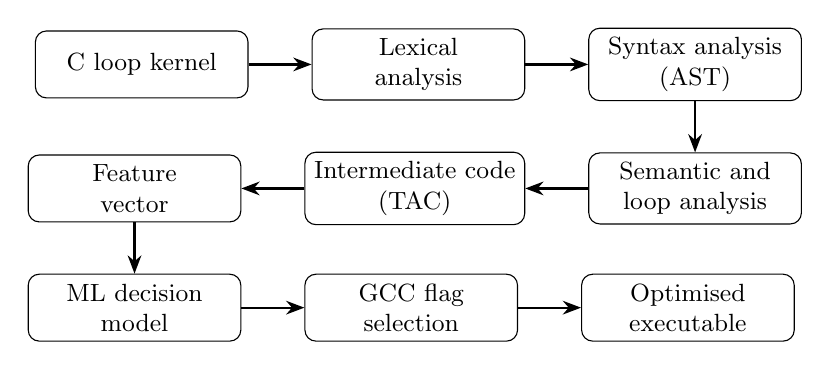
\begin{tikzpicture}[
node distance=0.65cm and 0.8cm,
box/.style={
rectangle,
rounded corners,
draw,
minimum width=2.7cm,
minimum height=0.85cm,
align=center,
font=\small
},
arrow/.style={-{Stealth},thick}
]

\node[box] (src) {C loop kernel};
\node[box,right=of src] (lex) {Lexical\\analysis};
\node[box,right=of lex] (syn) {Syntax analysis\\(AST)};
\node[box,below=of syn] (sem) {Semantic and\\loop analysis};
\node[box,left=of sem] (ir) {Intermediate code\\(TAC)};
\node[box,left=of ir] (feat) {Feature\\vector};
\node[box,below=of feat] (ml) {ML decision\\model};
\node[box,right=of ml] (flags) {GCC flag\\selection};
\node[box,right=of flags] (exe) {Optimised\\executable};

\draw[arrow] (src) -- (lex);
\draw[arrow] (lex) -- (syn);
\draw[arrow] (syn) -- (sem);
\draw[arrow] (sem) -- (ir);
\draw[arrow] (ir) -- (feat);
\draw[arrow] (feat) -- (ml);
\draw[arrow] (ml) -- (flags);
\draw[arrow] (flags) -- (exe);

\end{tikzpicture}

\caption{Proposed workflow: compiler front end, feature extraction and ML-based optimisation decision.}
\label{fig:workflow}
\end{figure}

\begin{figure}[H]
\centering
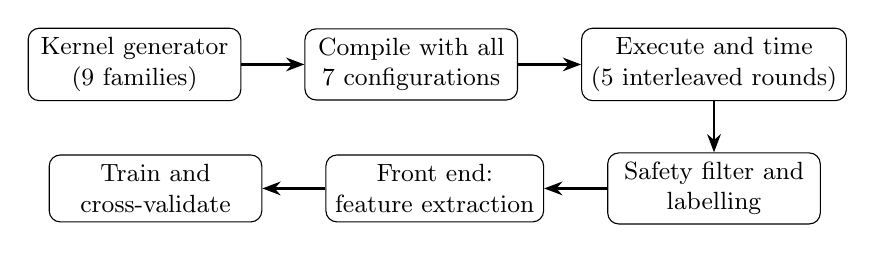
\begin{tikzpicture}[
node distance=0.65cm and 0.8cm,
box/.style={rectangle,rounded corners,draw,minimum width=2.7cm,minimum height=0.85cm,align=center,font=\small},
arrow/.style={-{Stealth},thick}
]
\node[box] (gen) {Kernel generator\\(\numFamilies\ families)};
\node[box,right=of gen] (comp) {Compile with all\\\numConfigs\ configurations};
\node[box,right=of comp] (time) {Execute and time\\(5 interleaved rounds)};
\node[box,below=of time] (lab) {Safety filter and\\labelling};
\node[box,left=of lab] (fe) {Front end:\\feature extraction};
\node[box,left=of fe] (train) {Train and\\cross-validate};
\draw[arrow] (gen) -- (comp);
\draw[arrow] (comp) -- (time);
\draw[arrow] (time) -- (lab);
\draw[arrow] (lab) -- (fe);
\draw[arrow] (fe) -- (train);
\end{tikzpicture}
\caption{Offline phase: construction of the labelled data set and training.}
\label{fig:offline}
\end{figure}

\subsection{Lexical Analysis}

Lexical analysis converts a sequence of characters into tokens. The scanner
(\texttt{lexer.py}) is specified by regular expressions in the same way as a
Lex/Flex description, with token classes \texttt{KEYWORD}, \texttt{TYPE},
\texttt{IDENT}, \texttt{NUMBER}, \texttt{OP}, \texttt{PUNCT}; comments,
white space and pre-processor lines are discarded and an illegal character is
reported as a lexical error. For example, the statement

\begin{verbatim}
C[i][j] += A[i][k]*B[k][j];
\end{verbatim}

is converted into the token sequence (as printed by the implemented scanner):

\begin{verbatim}
IDENT C | [ i ] [ j ] | OP += | IDENT A | [ i ] [ k ] |
OP * | IDENT B | [ k ] [ j ] | ;
\end{verbatim}

\subsection{Syntax Analysis}

Syntax analysis determines whether the token sequence conforms to the grammar
of the language. The output is an Abstract Syntax Tree (AST). The parser
(\texttt{loop\_parser.py}) is a recursive-descent (LL(1)) parser; expressions are
parsed by precedence climbing, which corresponds to the usual left-recursion-free
expression grammar:

\begin{align*}
E &\rightarrow T\,(\,(+\,|\,-)\,T\,)^{*} &
T &\rightarrow F\,(\,(*\,|\,/)\,F\,)^{*} \\
F &\rightarrow \mathit{NUM}\;|\;\mathit{ID}\,[\,E\,]^{*}\;|\;(\,E\,)\;|\;-F &
S &\rightarrow \texttt{for}\;(\dots)\;S\;|\;\texttt{if}\;(E)\;S\;[\texttt{else}\;S]\;|\;L\;\mathit{op}\;E\,;
\end{align*}

where $\mathit{op}\in\{=,+\!=,-\!=,*\!=,/\!=\}$ and $L$ is a scalar or an array element.
The AST nodes are \texttt{For}, \texttt{If}, \texttt{Assign}, \texttt{BinOp},
\texttt{UnOp}, \texttt{Index}, \texttt{Var}, \texttt{Num} and \texttt{Call}.
Syntax errors are reported with the offending token and line.

\subsection{Semantic and Loop Analysis}

Semantic analysis checks contextual constraints: every array is declared and used
with the declared number of subscripts, every identifier is declared, and loop
bounds are constant expressions that can be evaluated from the \texttt{\#define}
constants (a simple symbol table). On the checked AST, the analyser computes the
information that drives the optimisation decision.

\paragraph{Trip counts.} For \texttt{for (i = lo; i < hi; i += s)}, the trip count is
$\lceil (hi-lo)/s\rceil$; the iteration space of a nest is the product of the trip counts.

\paragraph{Affine subscripts and strides.} Each subscript is evaluated as an
affine function $a\,v+b$ of the innermost loop variable $v$ (the function is
checked to be linear by evaluating it at three points). For an array with
dimensions $S_0,\dots,S_{n-1}$ and subscripts $e_0,\dots,e_{n-1}$ with
coefficients $a_k$ in $v$, the memory stride of the reference (in elements) is
\begin{equation}
\mathrm{stride}_v = \sum_{k=0}^{n-1} a_k \prod_{m>k} S_m .
\end{equation}
A stride of 1 is a unit-stride (vectorisable, cache-friendly) access, a stride of 0 is
loop-invariant, and a large stride (e.g.\ $S_1=M$ when the \emph{row} index is the inner loop
variable) is a cache-hostile access that loop interchange could repair.

\paragraph{Loop-carried dependences.} For a write $W$ and a read $R$ of the same
array with equal coefficients $a$ and offsets $b_W$, $b_R$ in the innermost
variable, the dependence distance is
\begin{equation}
d = \frac{b_W - b_R}{a}.
\end{equation}
If $d>0$ the read uses a value written $d$ iterations earlier (a flow dependence of
distance $d$) and the loop cannot be vectorised with a vector length larger than $d$.

\paragraph{Reductions.} A scalar (or an array element that is invariant in the inner loop)
updated with \texttt{+=}, \texttt{*=} or \texttt{x = x + \dots} is a reduction. Floating-point
reductions can only be vectorised if the compiler may re-associate the additions,
which is not allowed under strict IEEE semantics.

\subsection{Intermediate Representation}

The AST of the loop body is lowered to three-address code (\texttt{tac.py}). Each
instruction has at most one operator; simple affine subscripts remain inline.
Three-address code for the body of the matrix-multiplication loop
\texttt{C[i][j] += A[i][k]*B[k][j]} is:

\begin{align}
t_1 &= C[i][j]\\
t_2 &= A[i][k]\\
t_3 &= B[k][j]\\
t_4 &= t_2 * t_3\\
t_5 &= t_1 + t_4\\
C[i][j] &= t_5
\end{align}

The number of TAC instructions of the innermost body is used as a feature
(\texttt{tac\_len}) and the TAC of the complete loop nest, including labels and
conditional jumps, can be printed by the tool (Section~\ref{sec:results}).

\subsection{Feature Vector}

The analyser produces the \numFeatures\ features of Table~\ref{tab:features}. They
describe the size of the iteration space, the arithmetic and memory work of the body,
the access pattern, the dependence structure and the working set.

\begin{table}[H]
\centering
\caption{Static loop features used by the decision model.}
\label{tab:features}
\footnotesize
\begin{tabularx}{\textwidth}{lX}
\toprule
\textbf{Feature} & \textbf{Meaning}\\
\midrule
\texttt{dtype\_bytes} & Size of the data type (4 = float, 8 = double)\\
\texttt{nest\_depth} & Depth of the loop nest\\
\texttt{inner\_trip\_log2}, \texttt{total\_iters\_log2} & $\log_2$ of the innermost trip count and of the total iterations\\
\texttt{n\_add}, \texttt{n\_mul}, \texttt{n\_div}, \texttt{n\_flops} & Floating-point operations per innermost iteration (address arithmetic excluded)\\
\texttt{n\_loads}, \texttt{n\_stores}, \texttt{n\_arrays} & Distinct array loads, stores and arrays per iteration\\
\texttt{n\_branches} & Number of \texttt{if} statements in the body\\
\texttt{n\_unit\_stride}, \texttt{n\_nonunit\_stride}, \texttt{n\_invariant} & Number of references with stride 1, stride $\neq$ 0,1 and stride 0\\
\texttt{max\_stride\_log2} & $\log_2$ of the largest absolute stride\\
\texttt{has\_reduction} & 1 if the body contains a reduction\\
\texttt{has\_carried\_dep}, \texttt{dep\_distance} & 1 if a loop-carried flow dependence exists, and its distance\\
\texttt{footprint\_log2} & $\log_2$ of the total size in bytes of the arrays touched\\
\texttt{bytes\_per\_iter}, \texttt{arith\_intensity} & Bytes moved per iteration and flops per byte\\
\texttt{tac\_len} & Number of TAC instructions in the loop body\\
\bottomrule
\end{tabularx}
\end{table}

\subsection{Decision Space}

The model chooses one of the \numConfigs\ GCC configurations of Table~\ref{tab:configs}.
They are ordered from conservative to aggressive: \texttt{O2} is the default baseline,
the \texttt{native} variants use the instruction set of the build machine (less portable),
and \texttt{O3\_fast\_native} additionally allows floating-point re-association
(\texttt{-ffast-math}), which changes numerical results.

\begin{table}[H]
\centering
\caption{Decision space: the seven candidate optimisation configurations.}
\label{tab:configs}
\small

\begin{tabular}{ll}
\toprule
\textbf{Class} & \textbf{GCC flags} \\
\midrule
\texttt{O2} & \texttt{-O2} \\
\texttt{O3} & \texttt{-O3} \\
\texttt{O2\_unroll4} & \texttt{-O2 -funroll-loops --param max-unroll-times=4} \\
\texttt{O2\_unroll8} & \texttt{-O2 -funroll-loops --param max-unroll-times=8} \\
\texttt{O3\_native} & \texttt{-O3 -march=native} \\
\texttt{O3\_unroll\_native} & \texttt{-O3 -funroll-loops -march=native} \\
\texttt{O3\_fast\_native} & \texttt{-O3 -march=native -ffast-math} \\
\bottomrule
\end{tabular}
\end{table}


\subsection{Labelling Rule}

Every kernel is compiled and executed with all configurations. Let $T_c$ be the
measured time of configuration $c$ and $r_c$ the checksum of the program output. A
configuration is \emph{admissible} if its result agrees with the baseline:
\begin{equation}
\frac{|r_c-r_{O2}|}{|r_{O2}|} \le 10^{-3}.
\end{equation}
The label is the most conservative admissible configuration whose time is within
$\tau=5\%$ of the fastest admissible one:
\begin{equation}
y = \min_{\text{order}}\{\,c \;:\; c\ \text{admissible},\ T_c \le (1+\tau)\min_{c'\ \text{adm.}} T_{c'}\,\}.
\end{equation}
The tolerance $\tau$ keeps the label stable under measurement noise
(Section~\ref{sec:results}), and the conservative ordering prefers portable, numerically safe
flags whenever a more aggressive flag brings no real gain.

\subsection{Decision Models}

Four supervised classifiers from scikit-learn \cite{pedregosa2011} are compared: a depth-limited
\emph{Decision Tree} (interpretable, depth 5), a \emph{Random Forest} \cite{breiman2001} with
300 trees, \emph{Gradient Boosting} (100 trees of depth 3) and \emph{k-NN} on standardised features
($k=5$, distance weighting). They are compared with four baselines that do not use the features:
always \texttt{O2}, always \texttt{O3}, always \texttt{O3\_native} and the majority class.

\subsection{Proposed Algorithm}

\begin{algorithm}[H]
\caption{ML-Based Loop Optimisation Decision}
\label{alg:compiler}
\begin{algorithmic}[1]

\Require Loop kernel source $S$; trained model $f$; configurations $C$
\Ensure Compiler flags for $S$

\State $tokens \gets \textsc{Lex}(S)$
\State $ast \gets \textsc{Parse}(tokens)$
\State Check declarations, subscripts and loop bounds (semantic analysis)
\State $nest \gets$ loop nest with the largest iteration space
\State Evaluate trip counts, strides, dependence distance, reductions
\State $tac \gets \textsc{LowerToTAC}(ast)$
\State $\phi \gets$ feature vector from $nest$, $tac$ and the array declarations
\State $c^{*} \gets f(\phi)$
\State \Return \textsc{Flags}$(c^{*})$

\end{algorithmic}
\end{algorithm}

\begin{algorithm}[H]
\caption{Construction of the Training Set and Model}
\label{alg:training}
\begin{algorithmic}[1]

\Require Kernel corpus $\mathcal{K}$; configurations $C$; tolerance $\tau$
\Ensure Trained model $f$

\For{each kernel $L\in\mathcal{K}$}
    \State $\phi(L) \gets$ \textsc{ExtractFeatures}$(L)$
    \For{each configuration $c\in C$}
        \State compile $L$ with $c$
    \EndFor
    \For{round $=1$ \textbf{to} 5}
        \For{each $c\in C$}
            \State run the binary of $c$, record $T$ and the checksum
        \EndFor
    \EndFor
    \State $T_c \gets$ minimum over the rounds
    \State $y(L) \gets$ label by the rule above
\EndFor
\State Train $f$ on $\{(\phi(L),y(L))\}$ and evaluate with cross-validation
\State \Return $f$

\end{algorithmic}
\end{algorithm}

\subsection{Implementation}

The software is organised as follows (all files are provided with this report):

\begin{table}[H]
\centering
\caption{Source files of the implementation.}
\label{tab:files}
\small
\begin{tabular}{ll}
\toprule
\textbf{File} & \textbf{Role}\\
\midrule
\texttt{lexer.py} & Phase 1: scanner\\
\texttt{loop\_parser.py} & Phase 2: recursive-descent parser, AST\\
\texttt{loop\_analyzer.py} & Phase 3: semantic and loop analysis, feature extraction\\
\texttt{tac.py} & Phase 4: three-address-code generator\\
\texttt{kernel\_gen.py} & Generator of the kernel corpus and timing harness\\
\texttt{benchmark.py} & Compile/execute under all configurations\\
\texttt{build\_dataset.py} & Features, timings, safety filter and labels\\
\texttt{train\_model.py} & Training and evaluation of the models\\
\texttt{predict.py} & Command-line advisor for a new loop\\
\texttt{make\_report\_assets.py} & Generates the tables and plots of this report\\
\bottomrule
\end{tabular}
\end{table}

\newpage

% ============================================================
% PAGE 12-15 -- RESULTS
% ============================================================
\section{Results and Discussion}
\label{sec:results}

All numbers in this section were produced by the code accompanying this report;
the tables and plots are generated automatically from the measured data.

\subsection{Dataset Preparation}

The corpus consists of \numKernels\ C kernels in \numFamilies\ families
(Table~\ref{tab:corpus}). Each kernel is generated by sweeping the data type
(\texttt{float}/\texttt{double}), the problem size, the number of operands, the
access stride, the loop order or the dependence distance. Every kernel was
compiled with all \numConfigs\ configurations (\numCompiles\ compilations) and
executed; for each configuration the binary was run in five interleaved rounds
(\numRuns\ executions in total), and each execution reports the minimum of five
timed trials.

\begin{table}[H]
\centering
\caption{Composition of the loop-kernel corpus.}
\label{tab:corpus}
\small

\begin{tabular}{llcrr}
\toprule
\textbf{Family} & \textbf{Loop pattern} & \textbf{Depth} & \textbf{Kernels} & \textbf{Footprint (bytes)} \\
\midrule
\texttt{axpy} & vector update $y_i=\sum w_jx^{(j)}_i+\dots$ & 1 & 36 & $2^{13}$--$2^{24}$ \\
\texttt{cond} & loop with data-dependent branch & 1 & 16 & $2^{13}$--$2^{23}$ \\
\texttt{dot} & dot product / norm (FP reduction) & 1 & 18 & $2^{12}$--$2^{23}$ \\
\texttt{matmul} & matrix product, loop orders ijk/ikj/jki & 3 & 24 & $2^{14}$--$2^{20}$ \\
\texttt{recur} & first-order recurrence $a_i=f(a_{i-d})$ & 1 & 24 & $2^{13}$--$2^{23}$ \\
\texttt{stencil1d} & 3- and 5-point 1-D stencil & 1 & 16 & $2^{13}$--$2^{23}$ \\
\texttt{stencil2d} & 5-point 2-D Jacobi stencil & 2 & 8 & $2^{15}$--$2^{22}$ \\
\texttt{strided} & non-unit-stride gather $x[s\,i]$ & 1 & 20 & $2^{15}$--$2^{26}$ \\
\texttt{traverse2d} & 2-D row/column sums, copy, transpose & 2 & 20 & $2^{17}$--$2^{24}$ \\
\textbf{Total} &  &  & \textbf{182} &  \\
\bottomrule
\end{tabular}
\end{table}


\subsection{System Requirements}

\begin{table}[H]
\centering
\caption{System used for the experiments.}
\begin{tabular}{ll}
\toprule
\textbf{Component} & \textbf{Value}\\
\midrule
Processor & \cpuModel\ (AVX2 and AVX-512 available)\\
Cores available & \numCpus\\
RAM & \memGB\ GB\\
Operating System & Ubuntu 24.04 (Linux)\\
Compiler & \gccVersion\\
Programming Language & C (kernels), Python 3.12 (front end, ML)\\
Libraries & NumPy, pandas, scikit-learn\\
\bottomrule
\end{tabular}
\end{table}

\subsection{Evaluation Process}

The approach is evaluated with the following metrics. Let $T_c(L)$ be the time of
loop $L$ with configuration $c$, $\hat c(L)$ the predicted configuration, and
$c^{\star}(L)$ the fastest admissible configuration (oracle).

\subsubsection{Execution Time and Speed-up}

\[
S(L)=\frac{T_{O2}(L)}{T_{\hat c(L)}(L)} ,\qquad
\mathrm{GM}=\Big(\prod_{L} S(L)\Big)^{1/N}
\]

If the predicted configuration would change the numerical result, the safe baseline
\texttt{O2} is used instead (S = 1).

\subsubsection{Oracle Gain}

\[
G=\frac{\ln \mathrm{GM}_{\text{model}}}{\ln \mathrm{GM}_{\text{oracle}}}\times100
\]

\subsubsection{Regret}

\[
R=\frac{1}{N}\sum_L\left(\frac{T_{\hat c(L)}(L)}{T_{c^{\star}(L)}(L)}-1\right)\times100
\]

\subsubsection{Classification Metrics}

Accuracy and macro-averaged F1 over the \numConfigs\ classes are also reported.
They are less informative than speed-up because many configurations have almost the
same performance for a given loop.

\subsubsection{Validation Protocols}

\emph{Random 5-fold cross-validation} (repeated five times) measures interpolation
between similar loops. \emph{Leave-one-family-out} (LOFO) trains on eight families
and tests on the ninth, which measures generalisation to a new kind of loop and is
the stricter test.

\subsection{Measurement Noise}

The experiments ran on a shared virtual machine, and timings of the \emph{same} binary
vary from process to process (probably through physical-page placement and
cache conflicts). Across the five rounds, the baseline time of a kernel had a median
range of \noiseSpreadMedian\% (maximum minus minimum). Because the reported time is the
minimum over the rounds, the residual noise is smaller: comparing the minimum of the
odd rounds with the minimum of the even rounds gives a median difference of
\noiseSplitMedian\% (90th percentile \noiseSplitNinety\%). The 5\% tie tolerance of the
labelling rule is therefore of the order of the noise, but not above it for all kernels,
and some labels, especially among near-equivalent configurations, are uncertain.
This is a limitation of the experiment, discussed in Section~\ref{sec:limits}.

\subsection{Labels and Static Configurations}

Table~\ref{tab:labels} shows how often each configuration is the label and how a
\emph{static} choice of that configuration would perform over the whole corpus.
No static configuration is best for every kernel (the oracle is above all of them), which is the reason to learn the decision, but the aggressive configurations are close to the oracle on average.

\begin{table}[H]
\centering
\caption{Label distribution and performance of each \emph{static} configuration over all kernels (speed-up w.r.t.\ \texttt{O2}; a configuration that changes the numerical result is replaced by \texttt{O2}).}
\label{tab:labels}
\small
\resizebox{\textwidth}{!}{%
\begin{tabular}{lrrrrr}
\toprule
\textbf{Config} & \textbf{Label count} & \textbf{Label \%} & \textbf{GM speed-up} & \textbf{Within 5\% of best} & \textbf{Rejected} \\
\midrule
\texttt{O2} & 25 & 13.7 & 1.000 & 25 & 0 \\
\texttt{O3} & 6 & 3.3 & 1.054 & 23 & 0 \\
\texttt{O2\_unroll4} & 2 & 1.1 & 1.084 & 26 & 0 \\
\texttt{O2\_unroll8} & 2 & 1.1 & 1.109 & 29 & 0 \\
\texttt{O3\_native} & 65 & 35.7 & 1.512 & 92 & 0 \\
\texttt{O3\_unroll\_native} & 37 & 20.3 & 1.560 & 114 & 0 \\
\texttt{O3\_fast\_native} & 45 & 24.7 & 2.197 & 128 & 0 \\
\textbf{Oracle} & -- & -- & \textbf{2.316} & -- & -- \\
\bottomrule
\end{tabular}}
\end{table}


\begin{figure}[H]
\centering
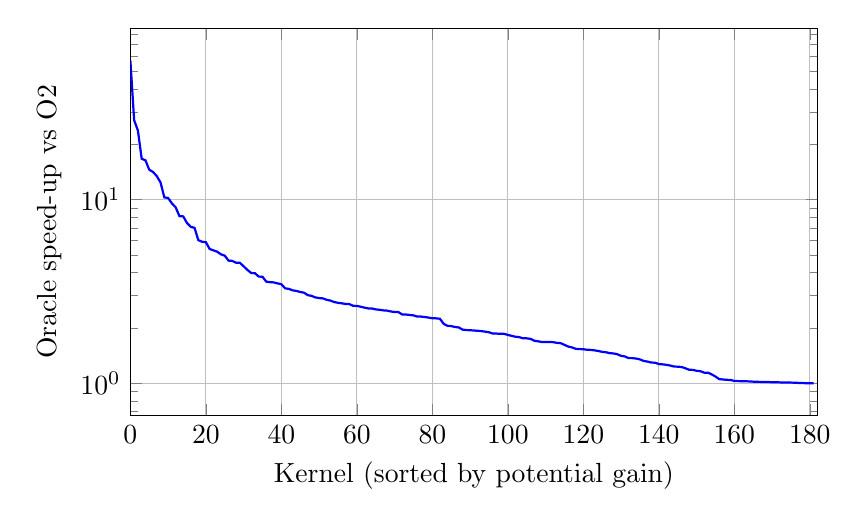
\begin{tikzpicture}
\begin{axis}[width=0.85\textwidth, height=6.5cm, xlabel={Kernel (sorted by potential gain)},
    ylabel={Oracle speed-up vs O2}, ymode=log, grid=major, xmin=0, xmax=182]
\addplot[thick, blue, no marks] coordinates {(0,57.256) (1,27.126) (2,23.777) (3,16.697) (4,16.376) (5,14.556) (6,14.146) (7,13.433) (8,12.393) (9,10.289) (10,10.210) (11,9.543) (12,9.080) (13,8.131) (14,8.106) (15,7.464) (16,7.109) (17,7.022) (18,6.018) (19,5.896) (20,5.866) (21,5.386) (22,5.293) (23,5.206) (24,5.037) (25,4.953) (26,4.655) (27,4.638) (28,4.532) (29,4.529) (30,4.336) (31,4.145) (32,3.986) (33,3.975) (34,3.810) (35,3.804) (36,3.575) (37,3.553) (38,3.541) (39,3.498) (40,3.464) (41,3.289) (42,3.265) (43,3.206) (44,3.182) (45,3.140) (46,3.113) (47,3.019) (48,2.991) (49,2.934) (50,2.910) (51,2.899) (52,2.848) (53,2.819) (54,2.768) (55,2.742) (56,2.725) (57,2.703) (58,2.699) (59,2.640) (60,2.638) (61,2.612) (62,2.581) (63,2.556) (64,2.553) (65,2.524) (66,2.513) (67,2.494) (68,2.486) (69,2.460) (70,2.442) (71,2.441) (72,2.369) (73,2.367) (74,2.354) (75,2.342) (76,2.307) (77,2.307) (78,2.294) (79,2.278) (80,2.259) (81,2.256) (82,2.245) (83,2.107) (84,2.055) (85,2.048) (86,2.024) (87,2.013) (88,1.959) (89,1.948) (90,1.945) (91,1.937) (92,1.931) (93,1.923) (94,1.910) (95,1.895) (96,1.866) (97,1.864) (98,1.859) (99,1.858) (100,1.834) (101,1.812) (102,1.792) (103,1.783) (104,1.757) (105,1.756) (106,1.745) (107,1.705) (108,1.692) (109,1.678) (110,1.678) (111,1.677) (112,1.674) (113,1.660) (114,1.653) (115,1.618) (116,1.584) (117,1.567) (118,1.540) (119,1.535) (120,1.532) (121,1.522) (122,1.519) (123,1.510) (124,1.498) (125,1.482) (126,1.475) (127,1.458) (128,1.453) (129,1.439) (130,1.410) (131,1.399) (132,1.370) (133,1.370) (134,1.363) (135,1.348) (136,1.322) (137,1.312) (138,1.296) (139,1.294) (140,1.272) (141,1.267) (142,1.260) (143,1.249) (144,1.233) (145,1.231) (146,1.226) (147,1.207) (148,1.185) (149,1.182) (150,1.169) (151,1.163) (152,1.142) (153,1.142) (154,1.118) (155,1.088) (156,1.053) (157,1.048) (158,1.044) (159,1.041) (160,1.030) (161,1.027) (162,1.026) (163,1.025) (164,1.023) (165,1.020) (166,1.018) (167,1.017) (168,1.017) (169,1.015) (170,1.013) (171,1.012) (172,1.011) (173,1.009) (174,1.009) (175,1.008) (176,1.007) (177,1.004) (178,1.003) (179,1.000) (180,1.000) (181,1.000)};
\end{axis}
\end{tikzpicture}
\caption{Best achievable speed-up over \texttt{O2} for each kernel (oracle).}
\label{fig:oracle}
\end{figure}


Figure~\ref{fig:oracle} shows the per-kernel gain that an oracle obtains over \texttt{O2}.
Many kernels gain from \texttt{-march=native}, because the machine supports AVX2 and
AVX-512 and the default \texttt{x86-64} target does not use them. Reductions
(\texttt{dot}) gain most from \texttt{-ffast-math}, which is consistent with the fact that
floating-point reductions can only be vectorised if the additions may be re-associated.
The other families show smaller but significant differences between the configurations.

\subsection{Performance of the Decision Models}

\begin{table}[H]
\centering
\caption{Comparison of decision models and static baselines. GM = geometric mean over kernels; ``Oracle gain'' is the share of the oracle's log-speed-up that is realised; ``Slow-downs'' counts kernels more than 5\% slower than \texttt{O2}.}
\label{tab:models}
\small
\resizebox{\textwidth}{!}{%
\begin{tabular}{llrrrrrr}
\toprule
\textbf{Model} & \textbf{Protocol} & \textbf{Acc.\ (\%)} & \textbf{Macro-F1} & \textbf{GM speed-up} & \textbf{Oracle gain (\%)} & \textbf{Regret (\%)} & \textbf{Slow-downs} \\
\midrule
Always -O2 & -- & 13.7 & 0.03 & 1.000 & 0 & 245.5 & 0 \\
Always -O3 & -- & 3.3 & 0.01 & 1.054 & 6 & 232.1 & 32 \\
Always -O3 -march=native & -- & 35.7 & 0.08 & 1.512 & 49 & 170.9 & 17 \\
Always -O3 -march=native -ffast-math & -- & 24.7 & 0.06 & 2.197 & 94 & 6.0 & 6 \\
Majority class & 5-fold CV & 35.7 $\pm$ 0.0 & 0.08 & 1.512 & 49 & 170.9 & 17 \\
Majority class & LOFO & 24.7 & 0.07 & 1.513 & 49 & 170.8 & 16 \\
Decision Tree & 5-fold CV & 60.7 $\pm$ 2.9 & 0.34 & 2.130 & 90 & 16.2 & 6 \\
Decision Tree & LOFO & 41.2 & 0.22 & 1.706 & 64 & 79.8 & 13 \\
Random Forest & 5-fold CV & 63.4 $\pm$ 1.0 & 0.38 & 2.221 & 95 & 4.9 & 6 \\
Random Forest & LOFO & 41.2 & 0.22 & 1.714 & 64 & 78.0 & 14 \\
Gradient Boosting & 5-fold CV & 60.2 $\pm$ 1.1 & 0.37 & 2.175 & 92 & 12.9 & 5 \\
Gradient Boosting & LOFO & 32.4 & 0.19 & 1.650 & 60 & 96.4 & 15 \\
k-NN & 5-fold CV & 66.5 $\pm$ 1.5 & 0.41 & 2.221 & 95 & 5.0 & 6 \\
k-NN & LOFO & 48.4 & 0.27 & 1.794 & 70 & 64.7 & 12 \\
\bottomrule
\end{tabular}}
\end{table}


Table~\ref{tab:models} and Figure~\ref{fig:speedup} compare the models with the static baselines. In random
cross-validation the learned models use the loop features well: the \selModel\ reaches \selAccCV\% accuracy and a
geometric-mean speed-up of \selGMCV, i.e.\ \selFracCV\% of the oracle gain (\oracleGM). Accuracy is only moderate
(macro-F1 \selFscoreCV) because several configurations perform within a few percent of each other; the speed-up is the
more relevant quantity.

The comparison with the \emph{best static configuration} is, however, sobering. Always compiling with
\texttt{-O3 -march=native -ffast-math} already gives \gmOFast, i.e.\ \fastFrac\% of the oracle gain, with a regret of
\fastRegret\% and \fastSlow\ slow-downs. The learned model (\selGMCV, regret \selRegretCV\%, \selSlowCV\ slow-downs) is
only marginally better in cross-validation. The reason is that on this processor, which has AVX2 and AVX-512 units,
the most aggressive flag set is the right choice for most of the kernels, so there is little left to decide. That static
choice is, however, not portable (it uses the instruction set of the build machine) and it relaxes IEEE floating-point
semantics; it passed the $10^{-3}$ checksum test on all kernels here, which does not prove that it is safe in general.

\begin{figure}[H]
\centering
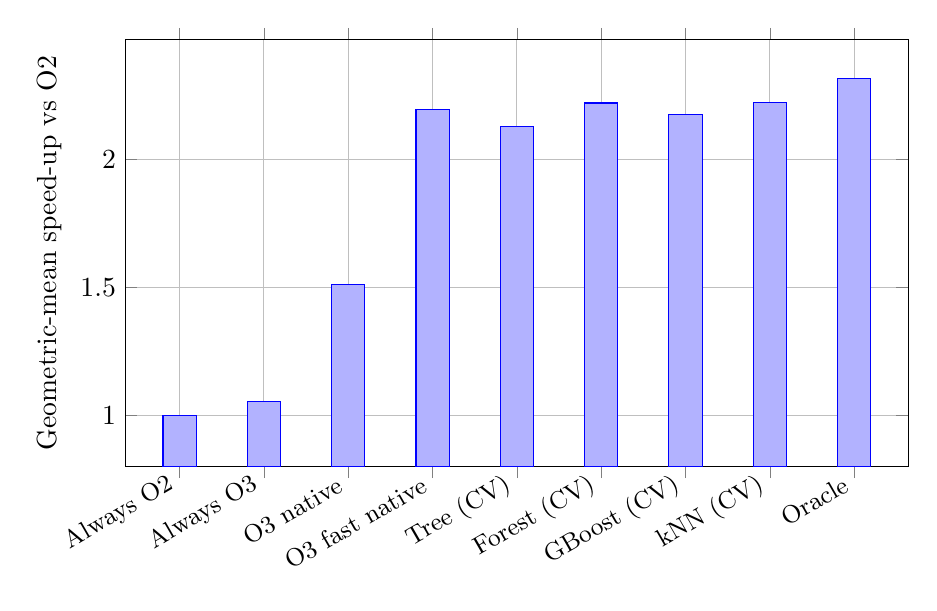
\begin{tikzpicture}
\begin{axis}[
    ybar, width=0.95\textwidth, height=7cm,
    ylabel={Geometric-mean speed-up vs O2},
    symbolic x coords={Always O2,Always O3,O3 native,O3 fast native,Tree (CV),Forest (CV),GBoost (CV),kNN (CV),Oracle},
    xtick=data, x tick label style={rotate=30,anchor=east,font=\small},
    ymin=0.8, 
    bar width=12pt,
    enlarge x limits=0.08,
    legend style={at={(0.5,1.03)},anchor=south,legend columns=-1,font=\small},
    grid=major]
\addplot coordinates {(Always O2,1.0000) (Always O3,1.0539) (O3 native,1.5122) (O3 fast native,2.1971) (Tree (CV),2.1300) (Forest (CV),2.2207) (GBoost (CV),2.1751) (kNN (CV),2.2215) (Oracle,2.3164)};

\end{axis}
\end{tikzpicture}
\caption{Geometric-mean speed-up over \texttt{O2} of the static configurations, the decision models (5-fold CV) and the oracle.}
\label{fig:speedup}
\end{figure}


Under leave-one-family-out the speed-up of the model falls to \selGMLOFO\ (\selFracLOFO\% of the oracle gain), the regret
rises from \selRegretCV\% to \selRegretLOFO\%, and the model is \emph{worse} than always choosing the aggressive
configuration (\gmOFast). Random splits overestimate the quality for new code because the corpus contains many close variants
of the same kernel. This is the main finding about the generalisation of the approach: with this corpus the model is not yet
reliable on a loop pattern that it has not seen.

\subsection{Portable Setting}

A more demanding decision arises when the program must run on any x86-64 machine and keep strict floating-point semantics.
The decision space is then restricted to \texttt{O2}, \texttt{O3}, \texttt{O2\_unroll4} and \texttt{O2\_unroll8}, and the
labels are recomputed from the same measurements with the same rule (Table~\ref{tab:portable}).

\begin{table}[H]
\centering
\caption{Portable setting: only the four IEEE-safe, non-native configurations (\texttt{O2}, \texttt{O3}, \texttt{O2\_unroll4}, \texttt{O2\_unroll8}) are allowed.}
\label{tab:portable}
\small
\resizebox{\textwidth}{!}{%
\begin{tabular}{llrrrrr}
\toprule
\textbf{Model} & \textbf{Protocol} & \textbf{Acc.\ (\%)} & \textbf{GM speed-up} & \textbf{Oracle gain (\%)} & \textbf{Regret (\%)} & \textbf{Slow-downs} \\
\midrule
Always -O2 & -- & 46.2 & 1.000 & 0 & 21.2 & 0 \\
Always -O3 & -- & 22.0 & 1.054 & 33 & 14.3 & 32 \\
Decision Tree & 5-fold CV & 51.9 & 1.088 & 53 & 9.0 & 5 \\
Decision Tree & LOFO & 37.4 & 1.012 & 7 & 19.6 & 8 \\
Random Forest & 5-fold CV & 52.1 & 1.102 & 60 & 7.3 & 7 \\
Random Forest & LOFO & 38.5 & 1.022 & 13 & 18.1 & 5 \\
k-NN & 5-fold CV & 57.1 & 1.108 & 64 & 6.6 & 6 \\
k-NN & LOFO & 43.4 & 1.039 & 23 & 15.8 & 3 \\
\textbf{Oracle} & -- & -- & \textbf{1.175} & 100 & 0.0 & 0 \\
\bottomrule
\end{tabular}}
\end{table}


Here the potential is smaller (oracle \pOracle), but the decision matters: always using \texttt{O3} gives \pOThree\ with
\pOThreeSlow\ kernels that become more than 5\% slower than \texttt{O2}. The \selModel\ reaches \pCV\ in cross-validation
(\pFracCV\% of the oracle gain) with \pSlowCV\ slow-downs on average, i.e.\ it keeps most of the benefit of \texttt{O3} while avoiding most of its
losses. Under leave-one-family-out it obtains \pLOFO\ (\pFracLOFO\% of the oracle gain) with \pSlowLOFO\ slow-downs: this is
slightly below the average speed-up of always using \texttt{O3}, but much safer.

\subsection{Per-Family Analysis}

\begin{table}[H]
\centering
\caption{Per-family geometric-mean speed-up over \texttt{O2} of the selected model (k-NN).}
\label{tab:family}
\small
\resizebox{\textwidth}{!}{%
\begin{tabular}{lrrrrrr}
\toprule
\textbf{Family} & \textbf{$n$} & \textbf{Oracle} & \textbf{Model (CV)} & \textbf{Model (LOFO)} & \textbf{Acc.\ CV (\%)} & \textbf{Acc.\ LOFO (\%)} \\
\midrule
\texttt{axpy} & 36 & 1.88 & 1.82 & 1.76 & 67 & 53 \\
\texttt{cond} & 16 & 5.02 & 4.98 & 1.29 & 81 & 6 \\
\texttt{dot} & 18 & 4.19 & 4.19 & 3.74 & 94 & 89 \\
\texttt{matmul} & 24 & 2.83 & 2.76 & 1.46 & 75 & 4 \\
\texttt{recur} & 24 & 1.38 & 1.26 & 1.27 & 54 & 42 \\
\texttt{stencil1d} & 16 & 1.73 & 1.67 & 1.67 & 50 & 81 \\
\texttt{stencil2d} & 8 & 2.26 & 2.23 & 2.21 & 25 & 75 \\
\texttt{strided} & 20 & 1.24 & 1.07 & 1.16 & 25 & 30 \\
\texttt{traverse2d} & 20 & 3.71 & 3.65 & 3.67 & 80 & 80 \\
\bottomrule
\end{tabular}}
\end{table}


\begin{figure}[H]
\centering
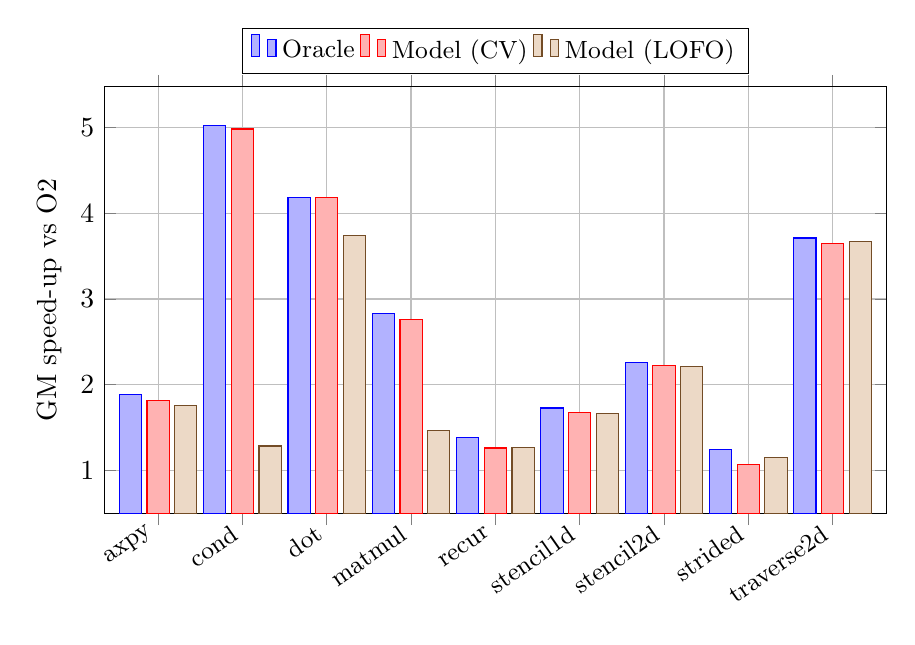
\begin{tikzpicture}
\begin{axis}[
    ybar, width=0.95\textwidth, height=7cm,
    ylabel={GM speed-up vs O2},
    symbolic x coords={axpy,cond,dot,matmul,recur,stencil1d,stencil2d,strided,traverse2d},
    xtick=data, x tick label style={rotate=35,anchor=east,font=\small},
    ymin=0.5, 
    bar width=8pt,
    enlarge x limits=0.08,
    legend style={at={(0.5,1.03)},anchor=south,legend columns=-1,font=\small},
    grid=major]
\addplot coordinates {(axpy,1.8813) (cond,5.0214) (dot,4.1862) (matmul,2.8279) (recur,1.3805) (stencil1d,1.7286) (stencil2d,2.2584) (strided,1.2434) (traverse2d,3.7099)};
\addplot coordinates {(axpy,1.8198) (cond,4.9817) (dot,4.1854) (matmul,2.7556) (recur,1.2621) (stencil1d,1.6731) (stencil2d,2.2253) (strided,1.0687) (traverse2d,3.6507)};
\addplot coordinates {(axpy,1.7556) (cond,1.2858) (dot,3.7438) (matmul,1.4649) (recur,1.2704) (stencil1d,1.6671) (stencil2d,2.2138) (strided,1.1561) (traverse2d,3.6741)};
\legend{Oracle,Model (CV),Model (LOFO)}
\end{axis}
\end{tikzpicture}
\caption{Per-family speed-up over \texttt{O2} for the k-NN: oracle, random-split cross validation, and leave-one-family-out.}
\label{fig:family}
\end{figure}


Table~\ref{tab:family} and Figure~\ref{fig:family} show that families with a clear structural signature
(\texttt{dot}, \texttt{traverse2d}, \texttt{matmul}, \texttt{cond}) are predicted nearly perfectly in
cross-validation. The \texttt{strided} family is the hardest: the best configuration depends on the
interaction of stride, cache size and the hardware prefetcher, which the static features describe only
roughly. In the leave-one-family-out test, \texttt{cond} and \texttt{matmul} lose most of their gain,
because no similar loop was in the training set: this indicates that the corpus must contain more
diverse loop patterns before the model can be trusted on new code. The families
\texttt{stencil1d}, \texttt{stencil2d}, \texttt{traverse2d} and \texttt{dot} transfer well because their
features resemble those of other families.

\subsection{Confusion Matrix and Feature Importance}

\begin{table}[H]
\centering
\caption{Confusion matrix of the k-NN (5-fold cross validation).}
\label{tab:confusion}
\scriptsize
\resizebox{\textwidth}{!}{%
\begin{tabular}{lrrrrrrr}
\toprule
\textbf{True $\backslash$ Pred} & \textbf{O2} & \textbf{O3} & \textbf{O2+unroll4} & \textbf{O2+unroll8} & \textbf{O3+native} & \textbf{O3+unroll+native} & \textbf{O3+fast+native} \\
\midrule
\textbf{O2} & 10 & 0 & 0 & 1 & 8 & 4 & 2 \\
\textbf{O3} & 1 & 2 & 0 & 0 & 2 & 1 & 0 \\
\textbf{O2+unroll4} & 0 & 0 & 0 & 0 & 0 & 2 & 0 \\
\textbf{O2+unroll8} & 1 & 0 & 0 & 0 & 1 & 0 & 0 \\
\textbf{O3+native} & 2 & 1 & 0 & 1 & 45 & 13 & 3 \\
\textbf{O3+unroll+native} & 5 & 0 & 1 & 0 & 6 & 22 & 3 \\
\textbf{O3+fast+native} & 0 & 0 & 0 & 0 & 5 & 3 & 37 \\
\bottomrule
\end{tabular}}
\end{table}


The confusion matrix (Table~\ref{tab:confusion}) shows that most errors are between neighbouring
aggressive configurations (for example \texttt{O3\_native} versus \texttt{O3\_unroll\_native}), whose
timing difference is small. Errors that choose a much slower configuration are rarer but produce the
slow-downs counted in Table~\ref{tab:models}.

\begin{figure}[H]
\centering
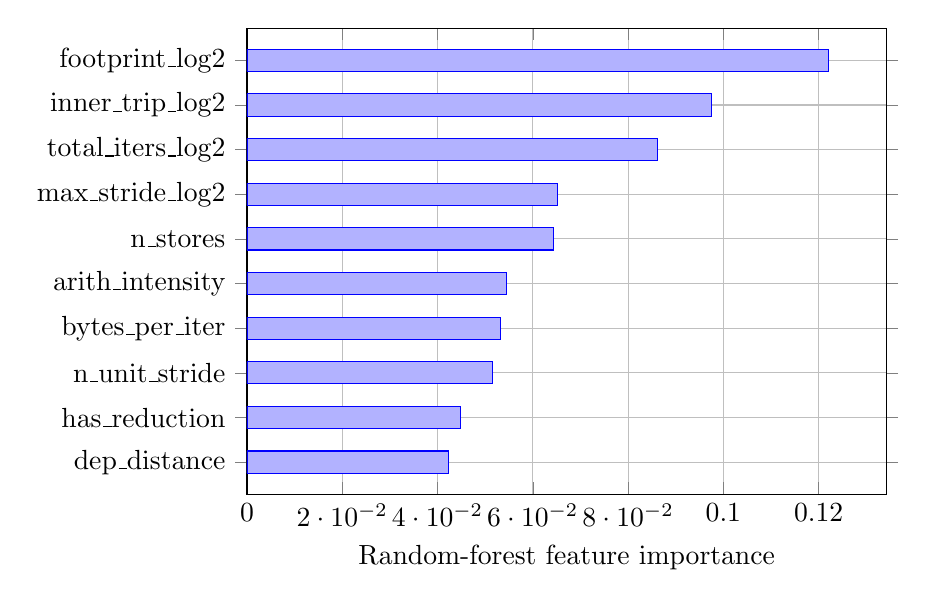
\begin{tikzpicture}
\begin{axis}[
    xbar, width=0.8\textwidth, height=7.5cm,
    xlabel={Random-forest feature importance},
    symbolic y coords={dep\_distance,has\_reduction,n\_unit\_stride,bytes\_per\_iter,arith\_intensity,n\_stores,max\_stride\_log2,total\_iters\_log2,inner\_trip\_log2,footprint\_log2},
    ytick=data, xmin=0, bar width=8pt, enlarge y limits=0.08, grid=major]
\addplot coordinates {(0.0423,dep\_distance) (0.0448,has\_reduction) (0.0515,n\_unit\_stride) (0.0532,bytes\_per\_iter) (0.0545,arith\_intensity) (0.0643,n\_stores) (0.0652,max\_stride\_log2) (0.0861,total\_iters\_log2) (0.0976,inner\_trip\_log2) (0.1220,footprint\_log2)};
\end{axis}
\end{tikzpicture}
\caption{Ten most important loop features.}
\label{fig:importance}
\end{figure}


Figure~\ref{fig:importance} shows that working-set size, trip counts and the largest memory stride
are the most important features. These are exactly the quantities that determine whether a loop is
bound by arithmetic, by cache or by memory bandwidth, and they are available from the
front end without running the program.

\subsection{Interpretable Rules}

A depth-5 decision tree trained on all data gives readable rules; the first levels are listed below
(\texttt{n\_stores}=0 identifies reductions, which are sent to \texttt{O3\_fast\_native}).

\lstinputlisting[language={},basicstyle=\ttfamily\scriptsize,numbers=none,lastline=26]{generated/decision_tree_rules.txt}

\subsection{Overhead of the Model}

Feature extraction takes about \featMs\ ms and prediction about \predMs\ ms per kernel, whereas a
single GCC compilation takes about \gccCompileMs\ ms on average. The decision is therefore of the same
order as, or cheaper than, one compiler run and is negligible compared with the search of an
iterative-compilation approach that compiles and runs every configuration (\numConfigs\ compilations per loop here).

\subsection{Sample Compiler Program}

The following C kernel (matrix product in the poor loop order j-k-i) is given to the advisor.
Note that this kernel is part of the training corpus, so the example illustrates the
tool and is not a test of generalisation.

\begin{lstlisting}
static DT A[M][M], B[M][M], C[M][M];   /* M = 96, DT = double */

DT kernel(int r)
{
    for (int j = 0; j < M; j++) {
        for (int k = 0; k < M; k++) {
            for (int i = 0; i < M; i++) {
                C[i][j] += A[i][k]*B[k][j];
            }
        }
    }
    return C[0][0];
}
\end{lstlisting}

\subsection{Lexical Analysis Output}

Token stream (first tokens of the loop, KIND:lexeme) for the kernel \texttt{cond\_double\_8192\_0p5\_1} printed by the scanner:

\lstinputlisting[language={},basicstyle=\ttfamily\small,numbers=none]{generated/tokens.txt}

\subsection{Three Address Code}

The loop nest of the same branchy kernel
(\texttt{if (x[i] > 0.5) y[i] = 0.5*x[i] + 0.1; else y[i] = 0.25*x[i];}) is lowered to the following
three-address code (before any optimisation; note the repeated loads of \texttt{x[i]}, which
common-subexpression elimination removes later):

\lstinputlisting[language={},basicstyle=\ttfamily\small,numbers=none]{generated/tac.txt}

\subsection{Advisor Output}

\lstinputlisting[language={},basicstyle=\ttfamily\scriptsize,numbers=none,firstline=1,lastline=5]{generated/predict_output.txt}
\lstinputlisting[language={},basicstyle=\ttfamily\scriptsize,numbers=none,firstline=29]{generated/predict_output.txt}

The feature vector, printed between these lines, shows the strides (96 elements for \texttt{C} and
\texttt{A}, i.e.\ a cache-hostile access), and the advisor selected \texttt{O2\_unroll4}, which was measured to be
faster than \texttt{-O2} for this kernel.

\subsection{Limitations and Threats to Validity}
\label{sec:limits}

\begin{itemize}
    \item \textbf{Single machine:} the labels depend on this processor. The large gains of the
    \texttt{native} configurations come from its AVX2/AVX-512 units; a different CPU requires re-labelling and re-training.
    \item \textbf{Synthetic corpus:} the kernels are small, regular HPC loops rather than whole applications, and similar
    kernels appear in several sizes. Random cross-validation is therefore optimistic, as the LOFO results show.
    \item \textbf{Timing noise:} on a shared virtual machine the residual noise (Section above) is comparable to the 5\% tie tolerance.
    \item \textbf{Numerical safety:} \texttt{-ffast-math} changes floating-point results. A configuration is only admissible if
    the checksum stays within a relative error of $10^{-3}$, which is a coarse test and is not a proof of correctness for other inputs.
    \item \textbf{Language subset:} the front end handles a C subset (affine subscripts, constant bounds, one function), not full C.
    \item \textbf{Portability:} binaries built with \texttt{-march=native} run only on processors with the same instruction set.
\end{itemize}

\newpage

% ============================================================
% PAGE 16 -- CONCLUSION
% ============================================================
\section{Conclusion and Future Work}

\subsection{Conclusion}

This report presented an ML-based loop-optimisation decision model built on a compiler
front end that was implemented from scratch. The lexical analyser, the recursive-descent parser,
the semantic and loop analyser and the three-address-code generator turn the source of a loop nest into
\numFeatures\ features (iteration space, memory strides, dependence distance, reductions,
arithmetic intensity, working set). A supervised model uses these features to select one of
\numConfigs\ GCC optimisation configurations.

The data set was measured and not simulated: \numKernels\ kernels were compiled with every configuration
and executed, and configurations that changed the numerical result were rejected. No static
configuration was best for all loops. With random cross-validation, the best model (\selModel) reached a
geometric-mean speed-up of \selGMCV\ over \texttt{-O2}, \selFracCV\% of the oracle's gain (\oracleGM). The honest reference is the
best static choice: always using \texttt{-O3 -march=native -ffast-math} gives \gmOFast\ on this machine, so the model
is only marginally better in cross-validation and worse (\selGMLOFO) on loop families that were not in the training set.
Where the binary has to be portable and IEEE-safe, the decision is more valuable: the model reached \pCV\ against \pOThree\ for
always using \texttt{-O3}, with far fewer slow-downs. Feature extraction and prediction cost less than one compiler invocation.

Overall, the study shows that the early compiler phases provide the information that optimisation decisions need,
and that a learned decision can replace a fixed heuristic, with two caveats: the training corpus must cover the
loop patterns that the model will meet, and on a machine where aggressive flags almost always win, a learned model adds
little over simply using them.

\subsection{Future Work}

Future work will focus on (i) a larger and more diverse corpus, including real benchmark loops (for example from
PolyBench), to close the gap between random and leave-one-family-out evaluation; (ii) a larger decision space with
loop-level choices such as tile size, unroll factor and interchange, implemented as source-to-source transformations on the
AST; (iii) repeating the experiment on several processors and adding machine features to the model; (iv) a more
robust measurement setup on a dedicated machine with fixed frequency; (v) active learning, in which the model
requests measurements only for loops it is unsure about; and (vi) integration with LLVM/MLIR passes.

\newpage

% ============================================================
% PAGE 17-18 -- REFERENCES
% ============================================================
\begin{thebibliography}{99}

\bibitem{aho2006}
A. V. Aho, M. S. Lam, R. Sethi, and J. D. Ullman,
\textit{Compilers: Principles, Techniques, and Tools},
2nd ed., Pearson/Addison-Wesley, 2006.

\bibitem{cooper2007}
K. D. Cooper and L. Torczon,
\textit{Engineering a Compiler},
2nd ed., Morgan Kaufmann, 2011.

\bibitem{appel2004}
A. W. Appel,
\textit{Modern Compiler Implementation in ML},
Cambridge University Press, 1998.

\bibitem{muchnick1997}
S. S. Muchnick,
\textit{Advanced Compiler Design and Implementation},
Morgan Kaufmann, 1997.

\bibitem{allen2002}
R. Allen and K. Kennedy,
\textit{Optimizing Compilers for Modern Architectures: A Dependence-Based Approach},
Morgan Kaufmann, 2002.

\bibitem{bacon1994}
D. F. Bacon, S. L. Graham, and O. J. Sharp,
``Compiler transformations for high-performance computing,''
\textit{ACM Computing Surveys}, vol. 26, no. 4, pp. 345--420, 1994.

\bibitem{wolf1991}
M. E. Wolf and M. S. Lam,
``A data locality optimizing algorithm,''
in \textit{Proc. ACM SIGPLAN Conference on Programming Language Design and
Implementation (PLDI)}, 1991, pp. 30--44.

\bibitem{bondhugula2008}
U. Bondhugula, A. Hartono, J. Ramanujam, and P. Sadayappan,
``A practical automatic polyhedral parallelizer and locality optimizer,''
in \textit{Proc. ACM SIGPLAN PLDI}, 2008, pp. 101--113.

\bibitem{wang2018}
Z. Wang and M. O'Boyle,
``Machine learning in compiler optimization,''
\textit{Proceedings of the IEEE}, vol. 106, no. 11, pp. 1879--1901, 2018.

\bibitem{ashouri2018}
A. H. Ashouri, W. Killian, J. Cavazos, G. Palermo, and C. Silvano,
``A survey on compiler autotuning using machine learning,''
\textit{ACM Computing Surveys}, vol. 51, no. 5, article 96, 2018.

\bibitem{stephenson2003}
M. Stephenson, S. Amarasinghe, M. Martin, and U.-M. O'Reilly,
``Meta optimization: improving compiler heuristics with machine learning,''
in \textit{Proc. ACM SIGPLAN PLDI}, 2003, pp. 77--90.

\bibitem{stephenson2005}
M. Stephenson and S. Amarasinghe,
``Predicting unroll factors using supervised classification,''
in \textit{Proc. International Symposium on Code Generation and Optimization (CGO)},
2005, pp. 123--134.

\bibitem{agakov2006}
F. Agakov, E. Bonilla, J. Cavazos, B. Franke, G. Fursin, M. F. P. O'Boyle,
J. Thomson, M. Toussaint, and C. K. I. Williams,
``Using machine learning to focus iterative optimization,''
in \textit{Proc. CGO}, 2006, pp. 295--305.

\bibitem{fursin2011}
G. Fursin et al.,
``Milepost GCC: Machine learning enabled self-tuning compiler,''
\textit{International Journal of Parallel Programming}, vol. 39, no. 3,
pp. 296--327, 2011.

\bibitem{cummins2017}
C. Cummins, P. Petoumenos, Z. Wang, and H. Leather,
``End-to-end deep learning of optimization heuristics,''
in \textit{Proc. International Conference on Parallel Architectures and
Compilation Techniques (PACT)}, 2017, pp. 219--232.

\bibitem{trofin2021}
M. Trofin, Y. Qian, E. Brevdo, Z. Lin, K. Choromanski, and D. Li,
``MLGO: a machine learning guided compiler optimizations framework,''
arXiv:2101.04808, 2021.

\bibitem{chen2018}
T. Chen et al.,
``TVM: An automated end-to-end optimizing compiler for deep learning,''
in \textit{Proc. USENIX Symposium on Operating Systems Design and
Implementation (OSDI)}, 2018, pp. 578--594.

\bibitem{lattner2021}
C. Lattner et al.,
``MLIR: Scaling compiler infrastructure for domain specific computation,''
in \textit{Proc. IEEE/ACM International Symposium on Code Generation and
Optimization (CGO)}, 2021.

\bibitem{abadi2016}
M. Abadi et al.,
``TensorFlow: A system for large-scale machine learning,''
in \textit{Proc. 12th USENIX Symposium on Operating Systems Design and
Implementation}, 2016, pp. 265--283.

\bibitem{pedregosa2011}
F. Pedregosa et al.,
``Scikit-learn: Machine learning in Python,''
\textit{Journal of Machine Learning Research}, vol. 12, pp. 2825--2830, 2011.

\bibitem{breiman2001}
L. Breiman,
``Random forests,''
\textit{Machine Learning}, vol. 45, no. 1, pp. 5--32, 2001.

\bibitem{gcc}
Free Software Foundation,
\textit{Using the GNU Compiler Collection (GCC)},
GCC Online Documentation.

\end{thebibliography}

\end{document}
